\chapter{Experiments}
\section{Low Dimensional Reward Bounds}
\subsection{Simulation Setup}
\begin{figure}[h]
	\centering
	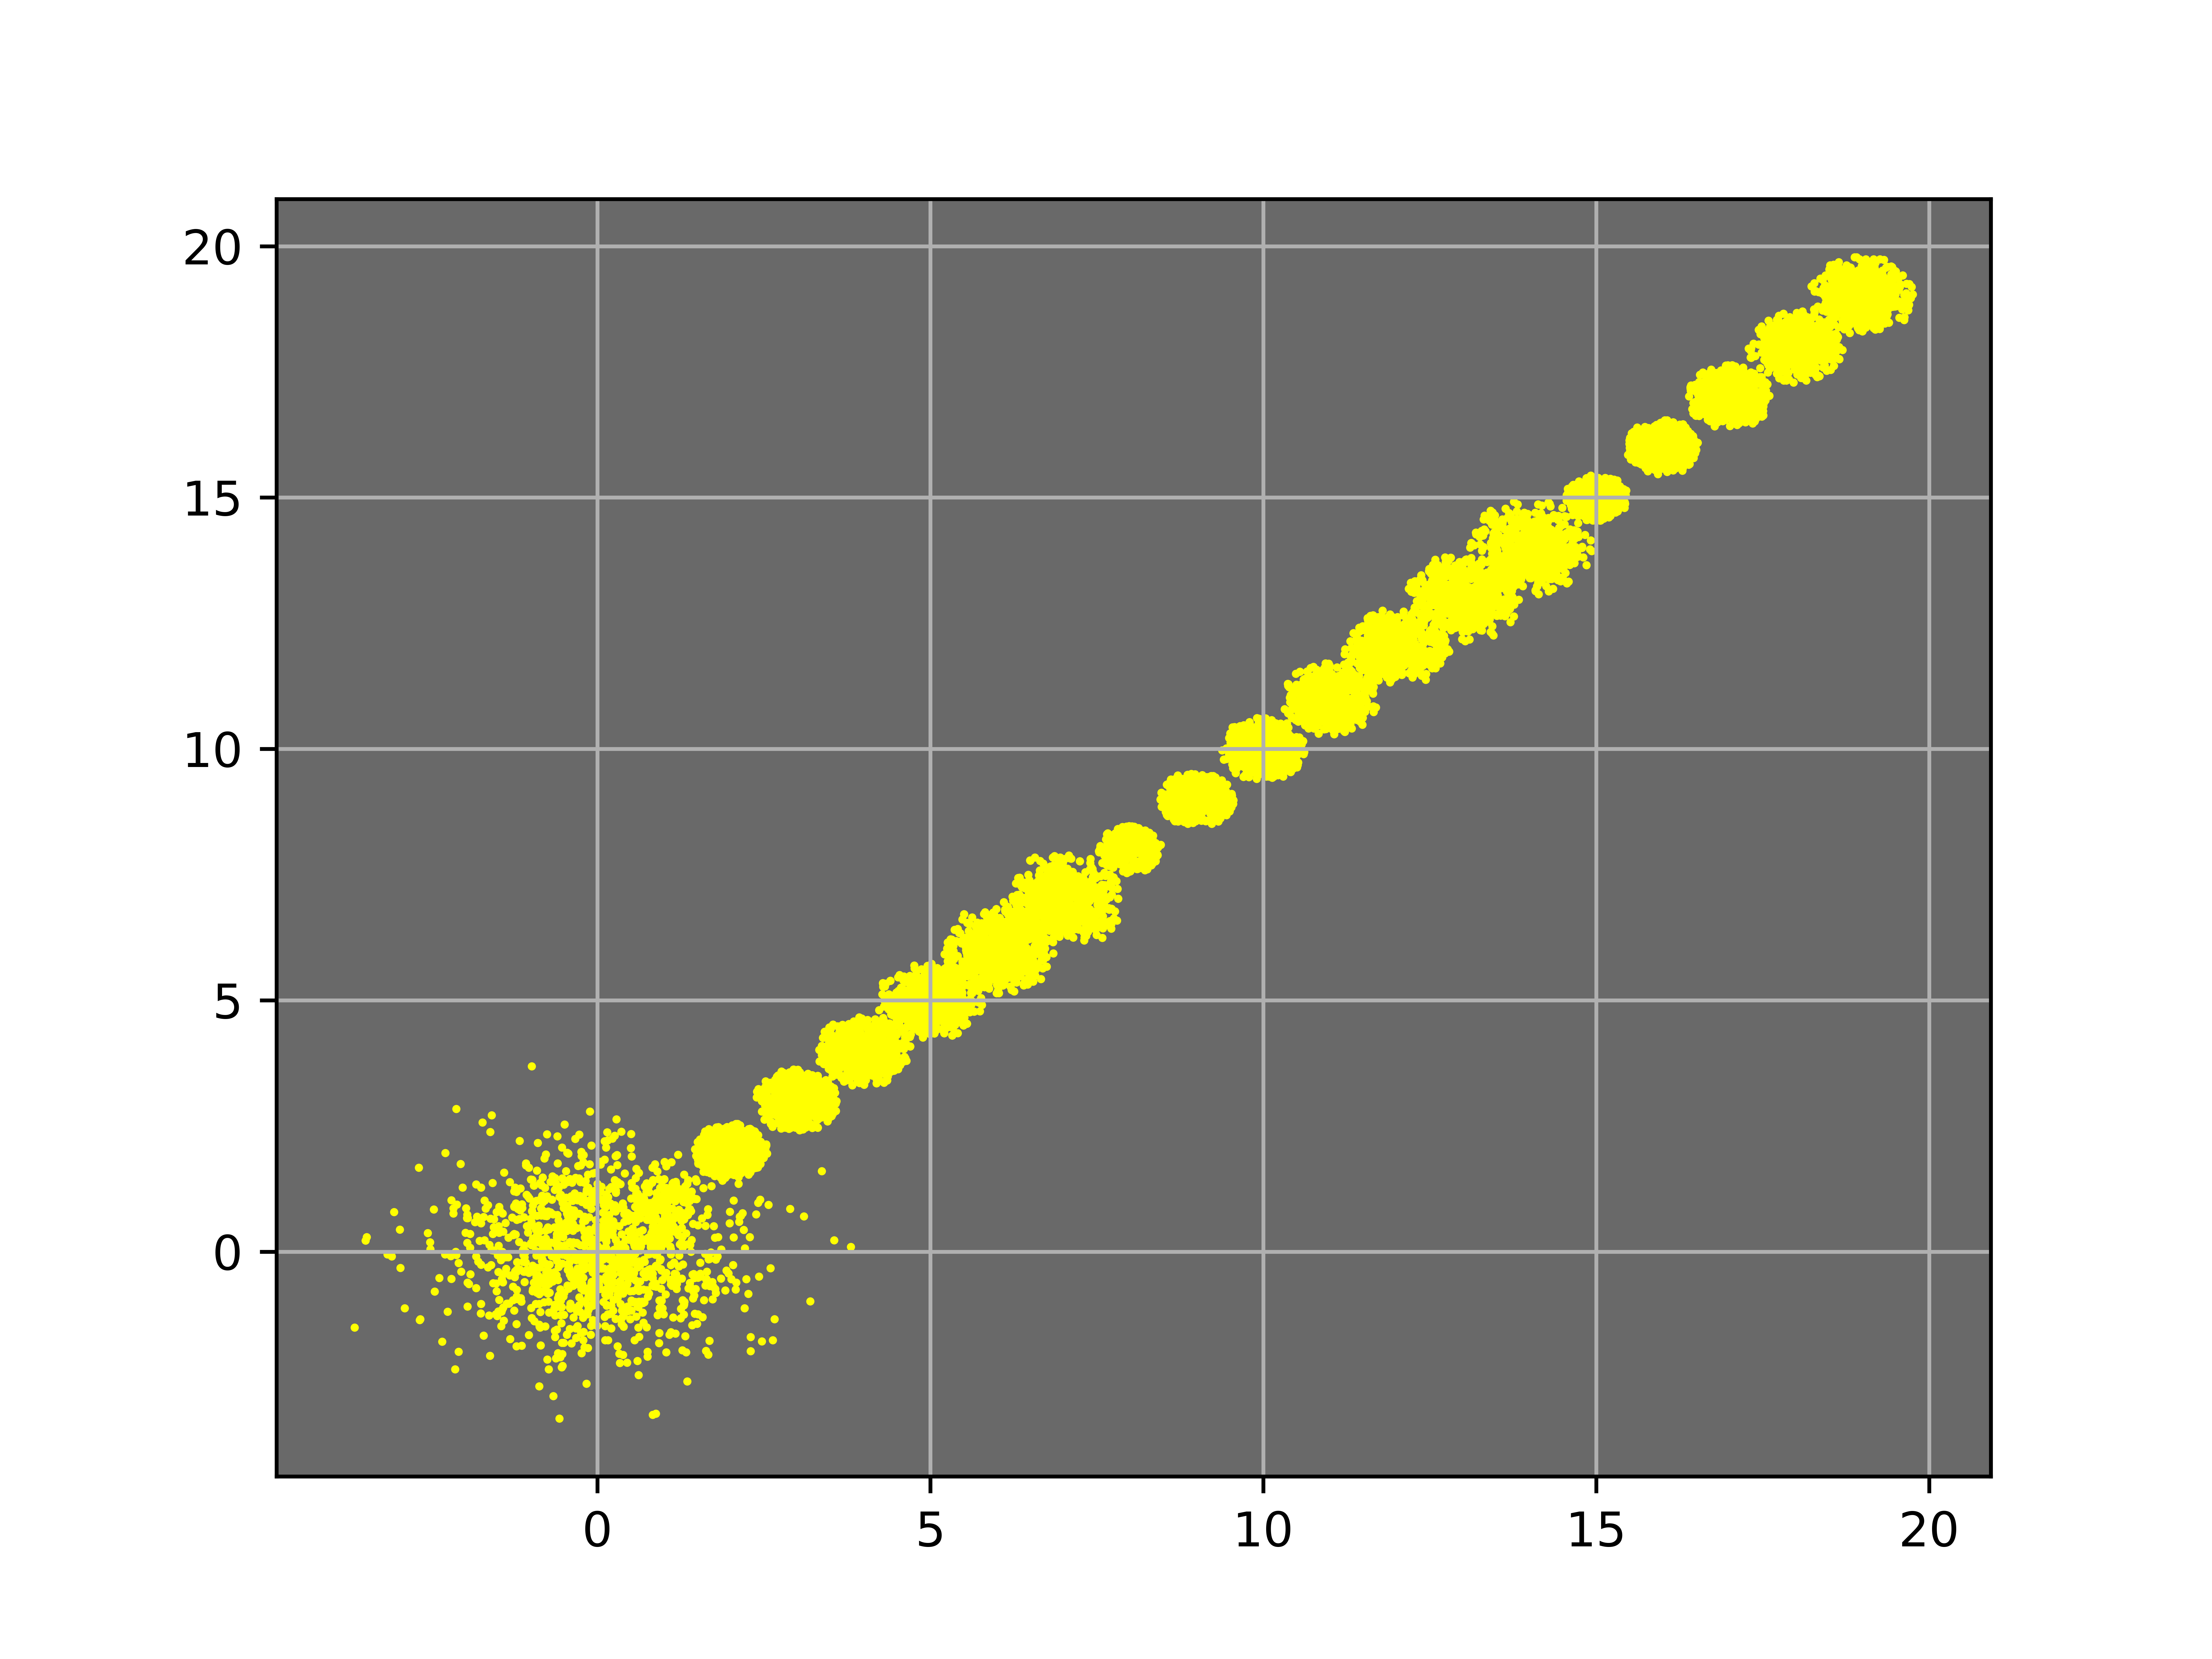
\includegraphics[width= 0.4\linewidth,clip]{belief_trajectory}
	\caption{The trajectory of the particle filter over time. The action taken each time-step is $[1,1]$.}
	\label{fig:belief_trajectory}
\end{figure}
	We begin our empirical study in a low dimensional particle filter scenario. The agent is given to be in $\mathbb{R}^2$, and we begin with a prior belief $\blf{0}\sim N(0,I\sigma_0^2)$. The agent is moved along a predetermined trajectory for which it is given a transition model upon which to perform predictions of the form $\state{}^\prime=\state{}+\action{}+\omega_{\action{}}$ where $\omega_{\action{}}\sim N_{r_a}(0,I\sigma_{\action{}}^2)$. The agent also gathers noisy measurements along its path $\observation{}{}=\state{}+\omega_{\observation{}{}}$, where $\omega_{\observation{}{}}\sim N_{r_{\observation{}{}}}(0,I\sigma_{\observation{}{}}^2)$ and the observation noise is time dependent. $N_{r}(0,\Sigma)$ is a multivariate zero-mean Gaussian distribution with covariance $\Sigma$ and truncated at radius $r$, allowing for an infimum greater than zero, which is reasonable given noise filtering and outlier pruning practices. The belief is maintained as a set of weighted particles $\{\states{}^i,\weight{}{i}\}_{i=1}^N$ and we use a particle filter to update the belief each time-step. The reward is an estimator of the entropy given by~\cite{Boers10fusion}. At the end of each update step particles with zero weight were discarded (possible because of the truncated Gaussian), after reward calculation resampling was performed. The trajectory of the particle filter can be seen in \cref{fig:belief_trajectory}. We evaluate our bounds \autoref{thm:boers_bounds_simple} and compare them to those provided by~\cite{Sztyglic22iros}.
\subsection{Results}
\begin{figure}[h]
	\centering
	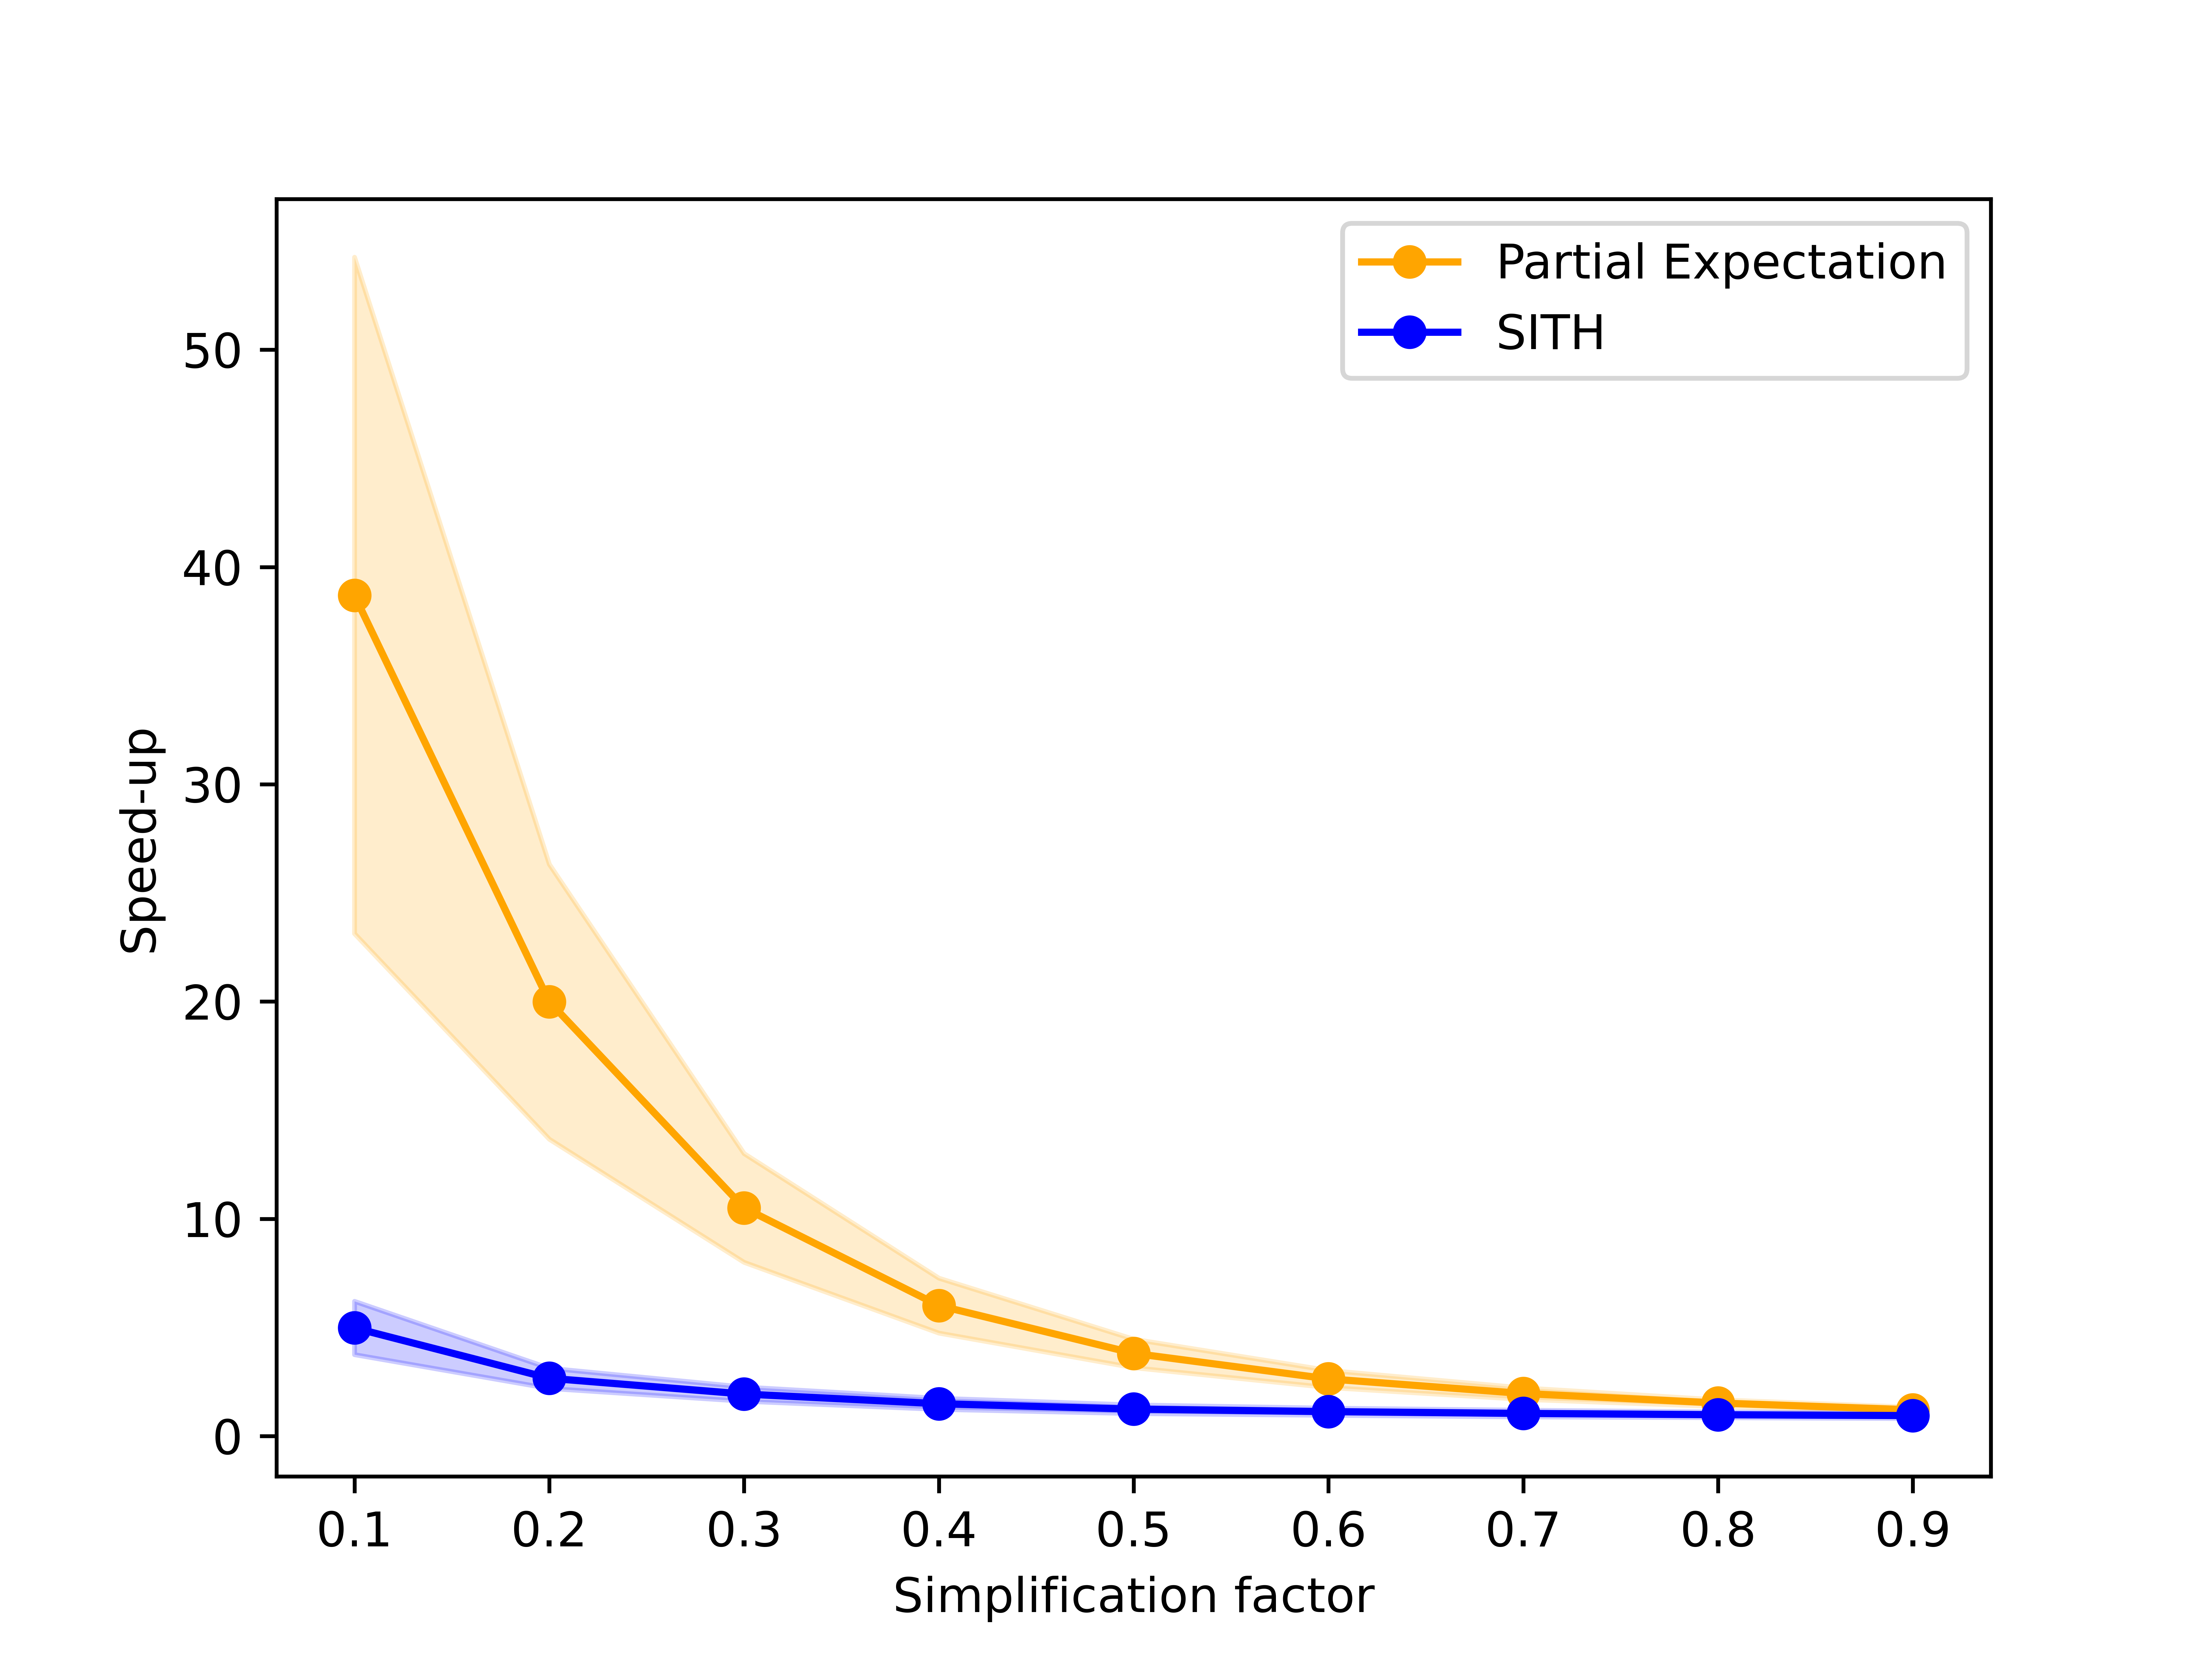
\includegraphics[width= 0.4\linewidth,clip]{speedup}
	\caption{The relative speed-up of each bounding algorithm on the Boer's estimator, speed-up is relative to the Boer's estimator time. Results are averaged over 10 runs using a nominal set of 1000 belief particles.}
	\label{fig:speedup}
\end{figure}
	In our comparison there are two primary aspects which we would like to investigate. This first is the relative computational efficiency of each algorithm, and the second is the bound tightness. Beginning with the computational efficiency, the Boer's estimator requires $O(N^2)$ computations. We define $\alpha = n/N$ to be the simplification factor, as such the computational complexity of the SITH bounds are $\alpha_sN^2$ and the complexity of our bounds are $\alpha_p^2N^2$ for $0<\alpha\leq1$. Thus for the same level of simplification, we expect a quadratic speed-up, whereas the SITH bounds are limited to a linear speed-up. If we look at \cref{fig:speedup} we observe this exact behavior. Furthermore, as the SITH algorithm also makes use of computations on the complementary set of particles is complexity has some added linear complexity with respect to $N$, this is often observed at large values of $\alpha$ where there is not much simplification. For example, for $\alpha_s=\numlist{0.8;0.9}$ the relative speed-up is less than 1, meaning that calculating the bounds is more computationally expensive.
\begin{figure} [h]
	\centering
	\begin{subfigure}[t]{0.32\textwidth}
		\centering
		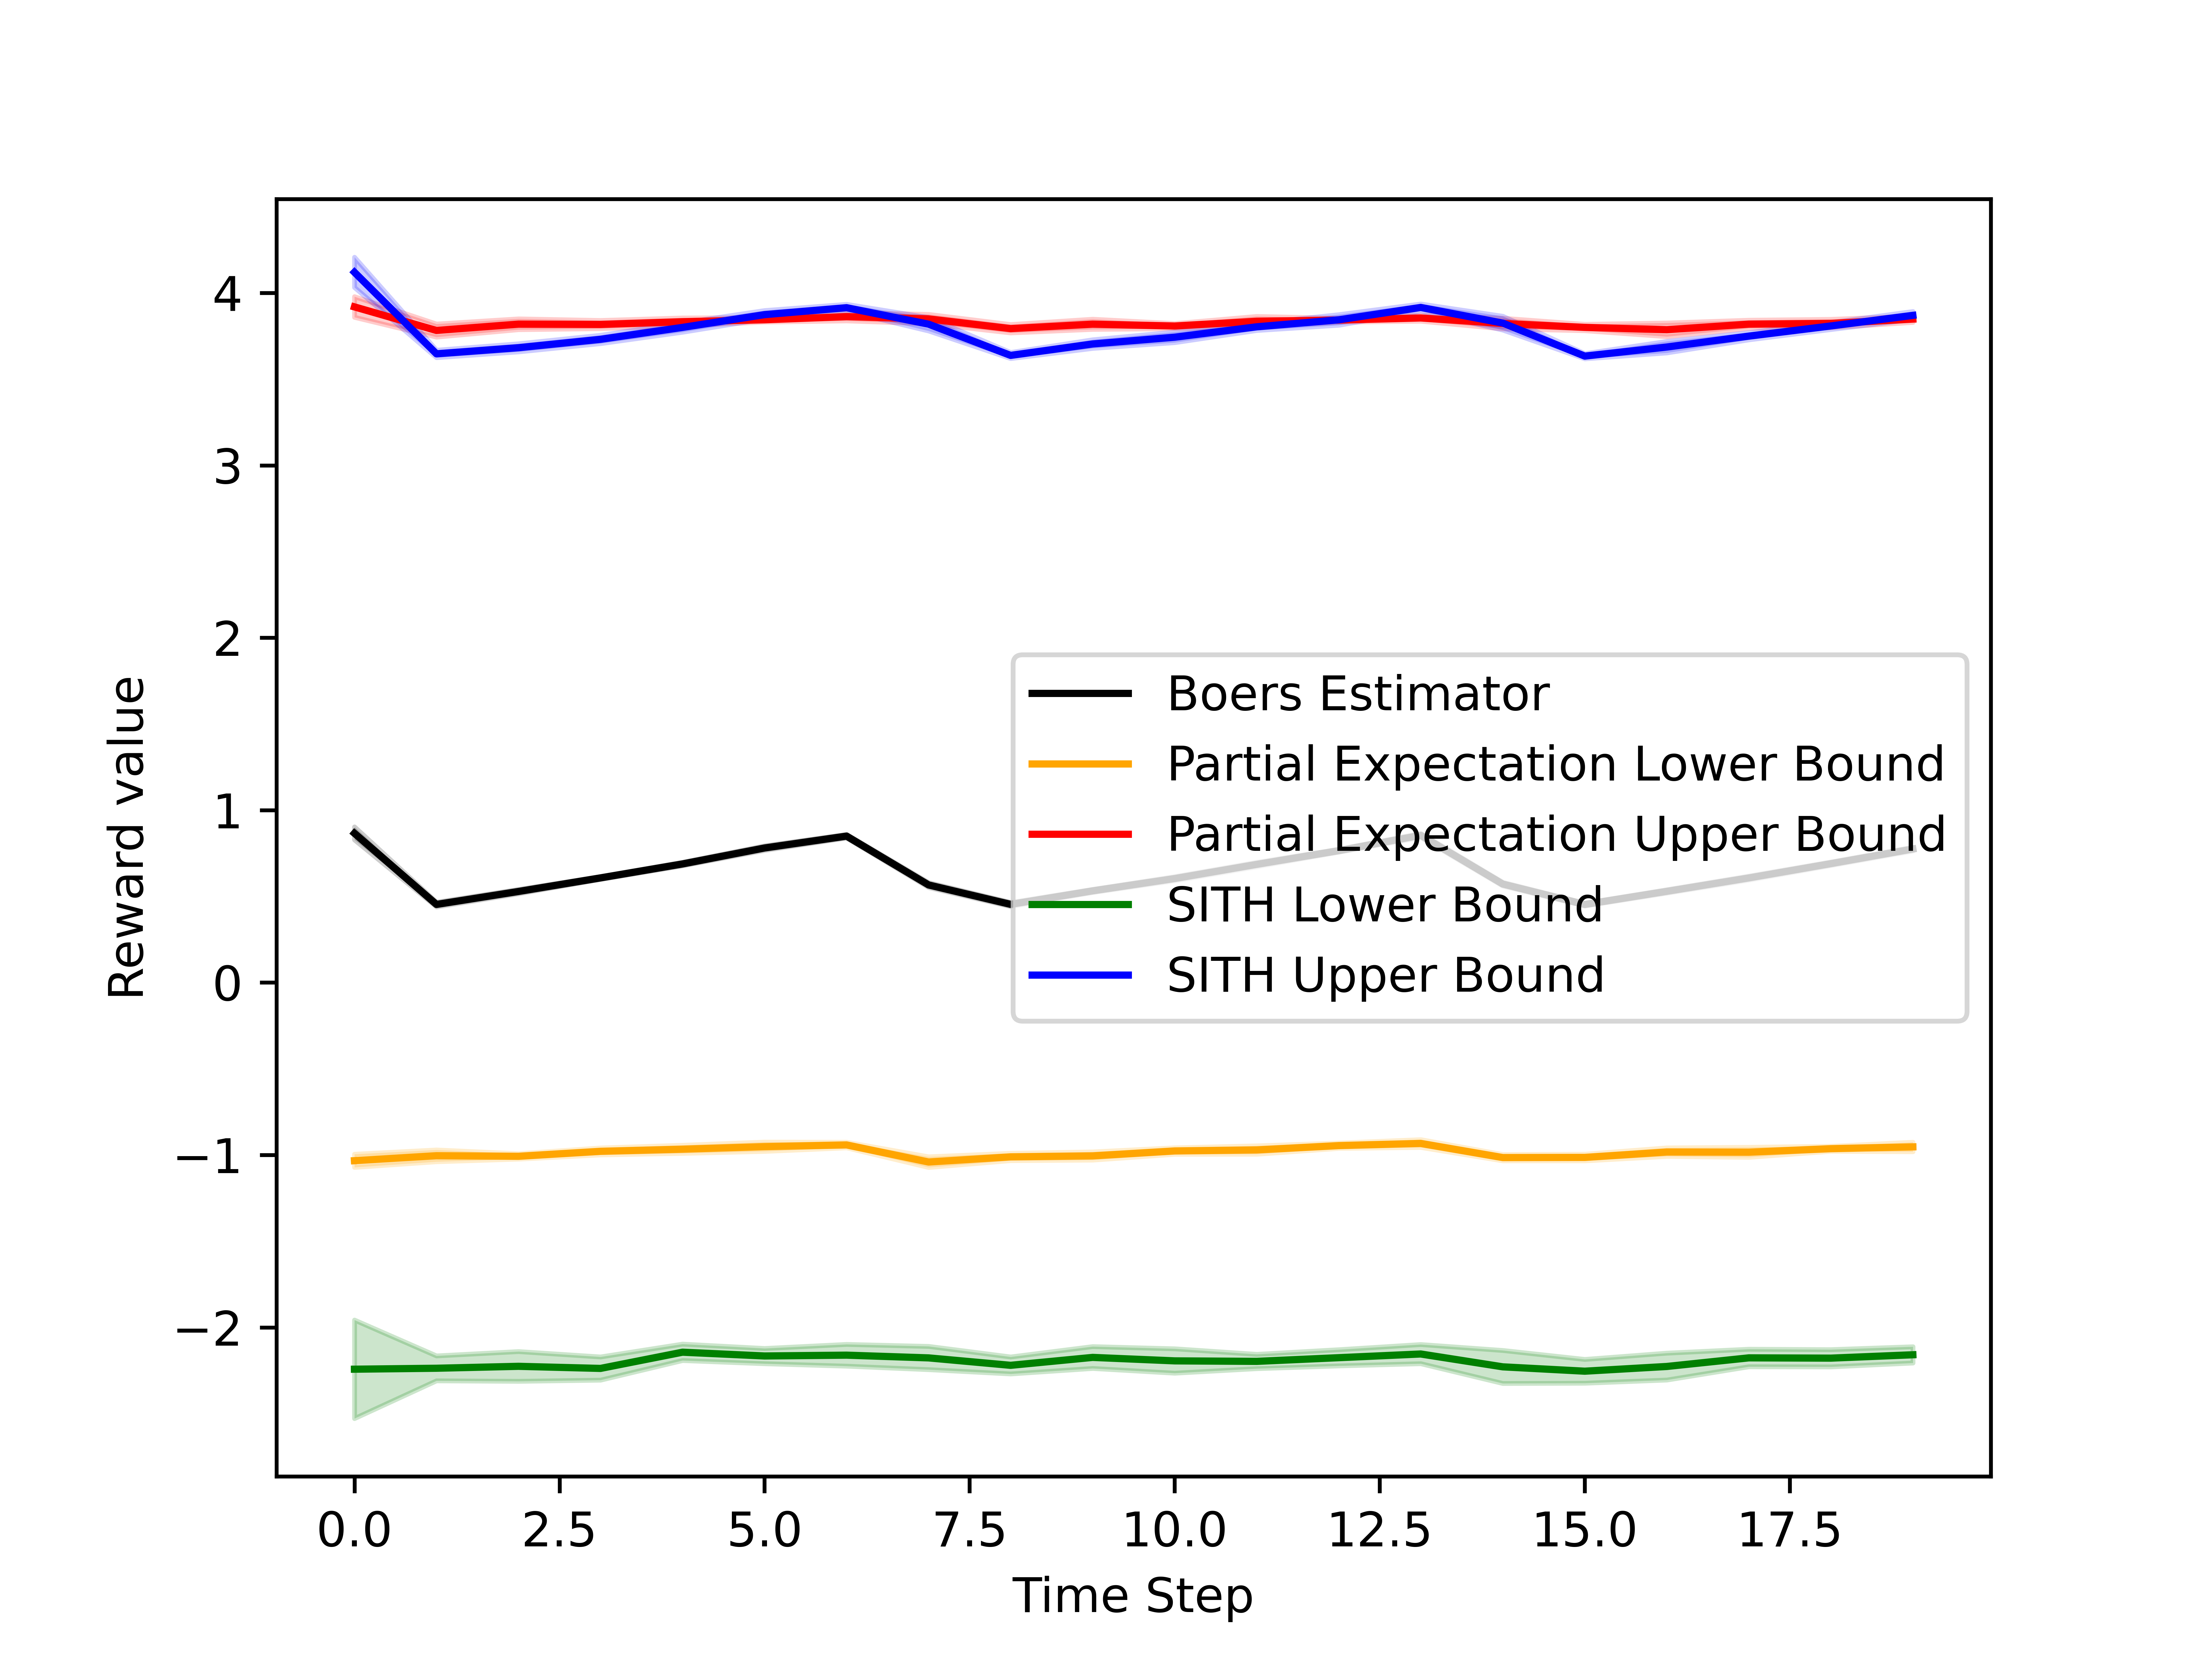
\includegraphics[width= 0.95\linewidth,clip]{1200_03}
		\caption{$\alpha_p=0.3$, relative speed-up of \num{11.0\pm2.7} for partial expectation and \num{5.8\pm1.5} for SITH}
		\label{fig:alpha_03}
	\end{subfigure}
	\hfill
	\begin{subfigure}[t]{0.32\textwidth}
		\centering
		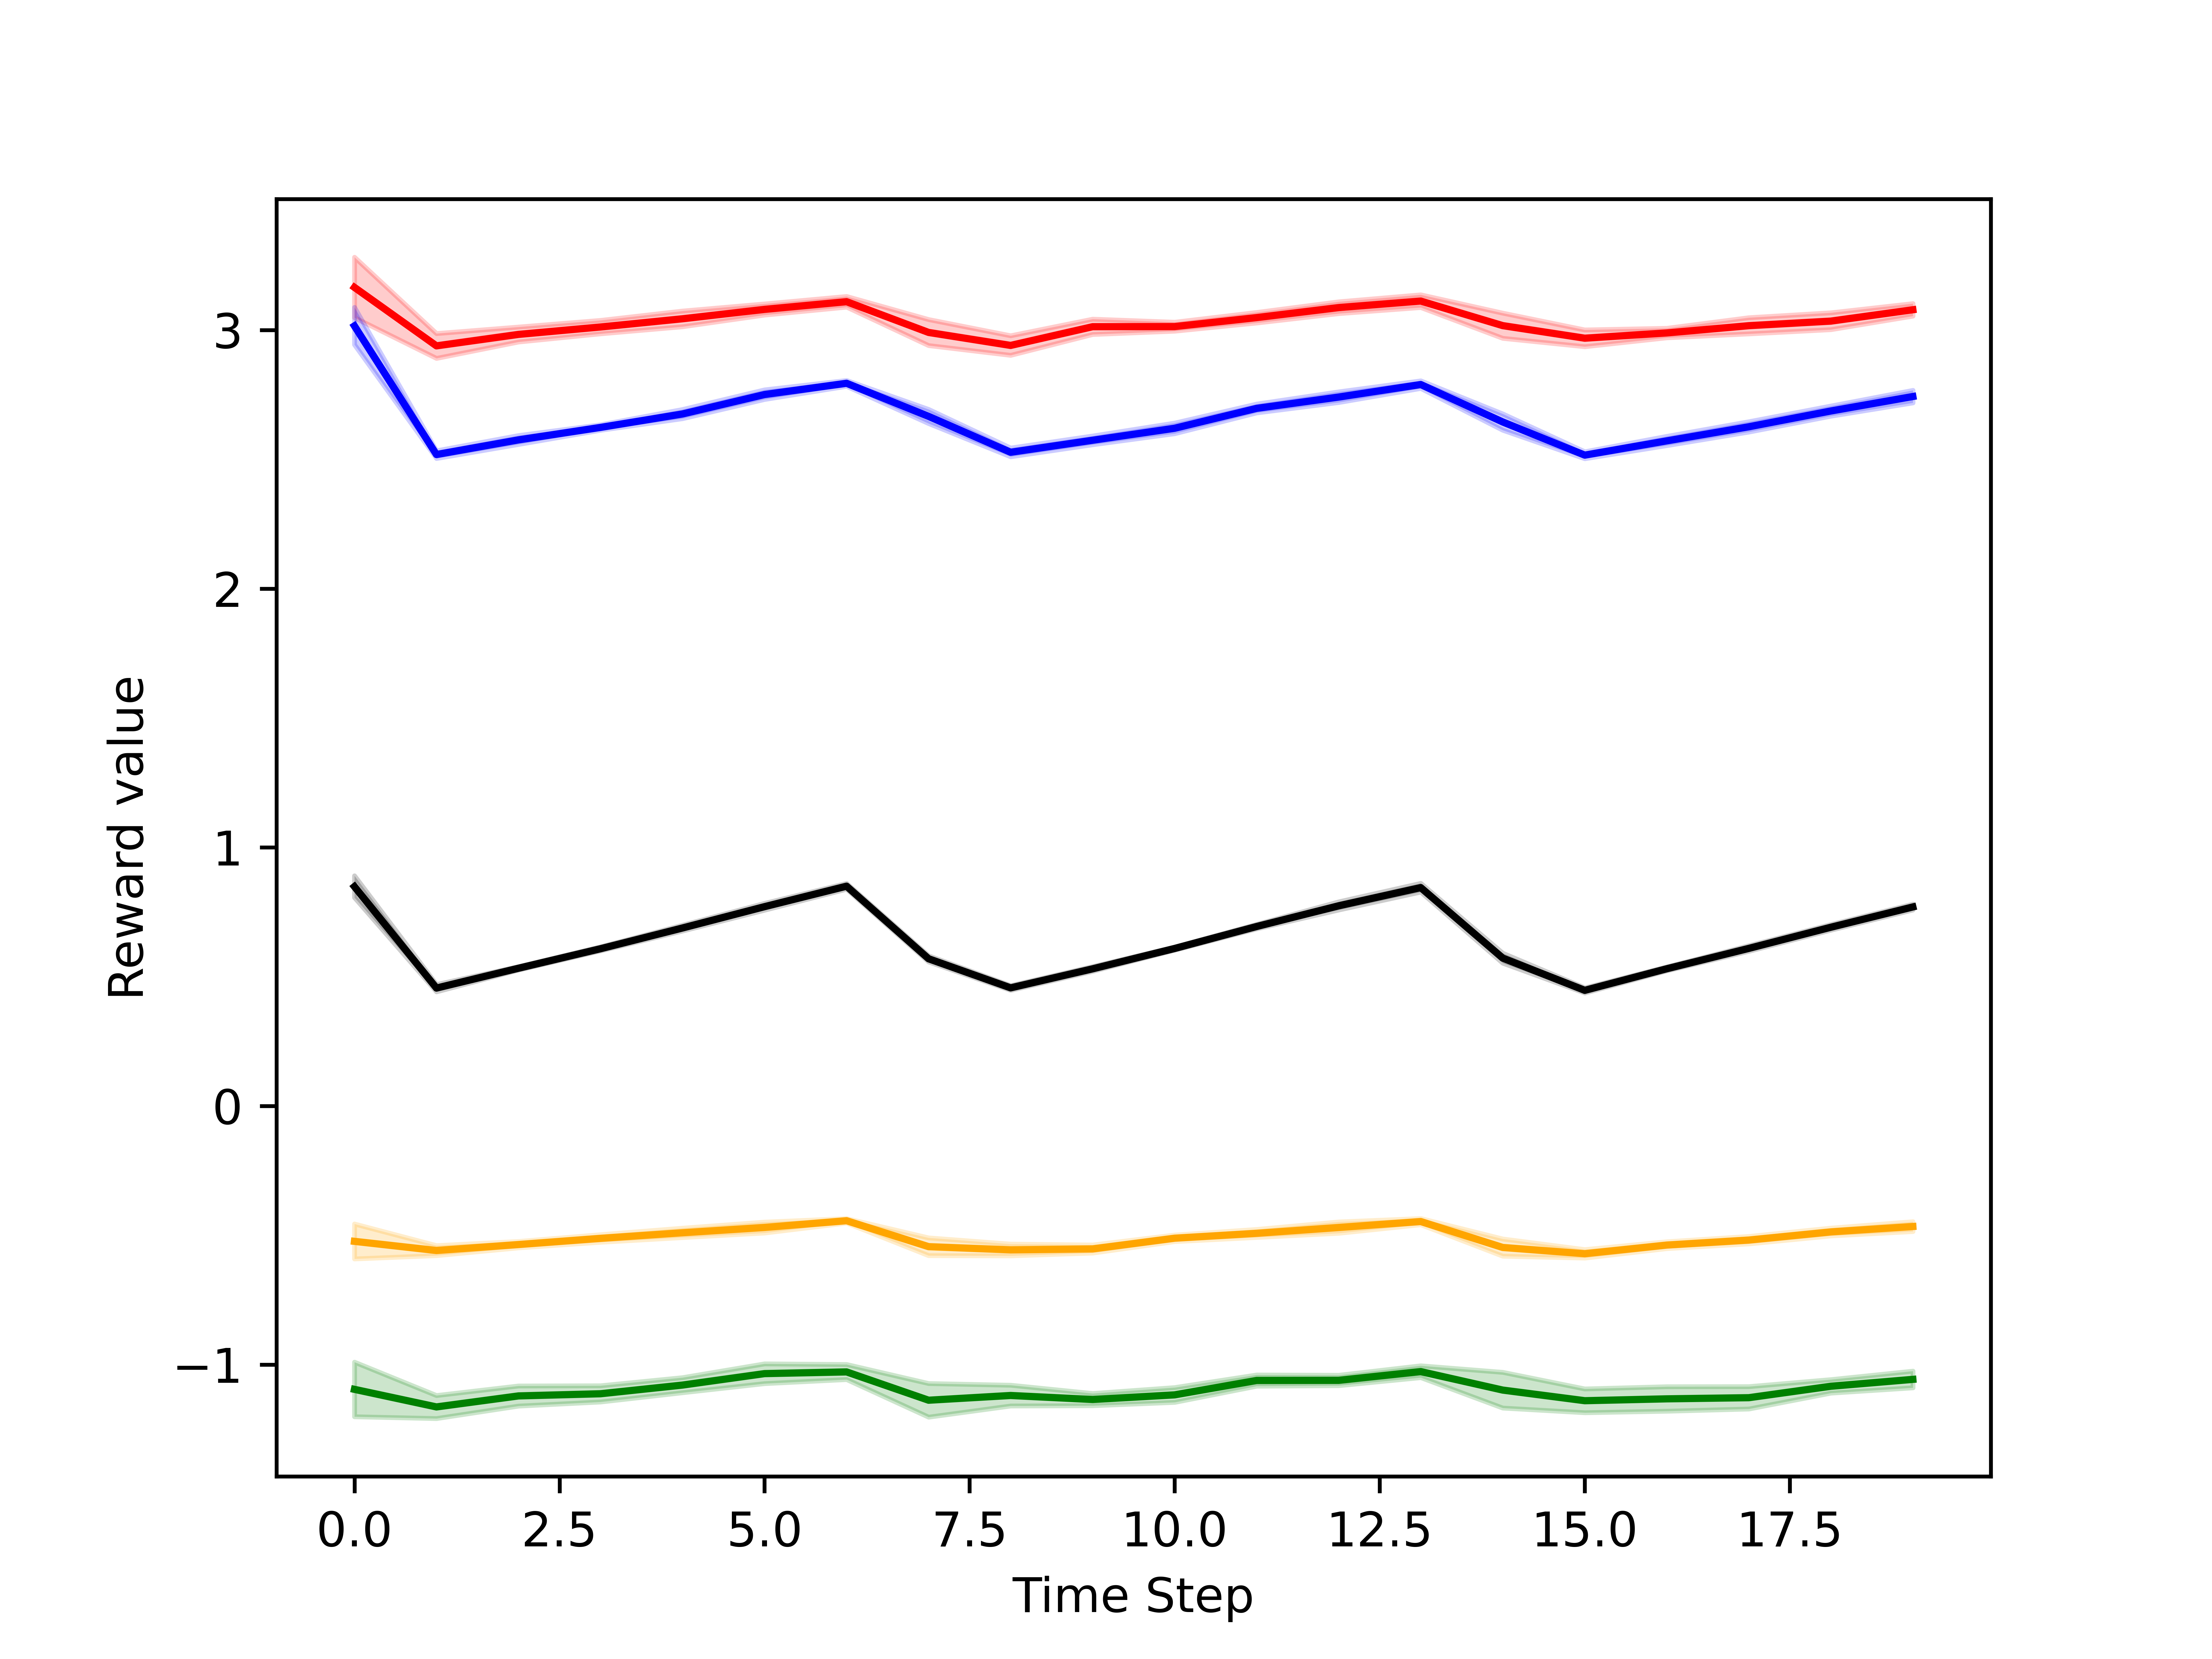
\includegraphics[width= 0.95\linewidth,clip]{1200_05}
		\caption{$\alpha_p=0.5$, relative speed-up of \num{3.6\pm0.5} for partial expectation and \num{2.0\pm0.3} for SITH}
		\label{fig:alpha_05}
	\end{subfigure}
	\hfill
	\begin{subfigure}[t]{0.32\textwidth}
		\centering
		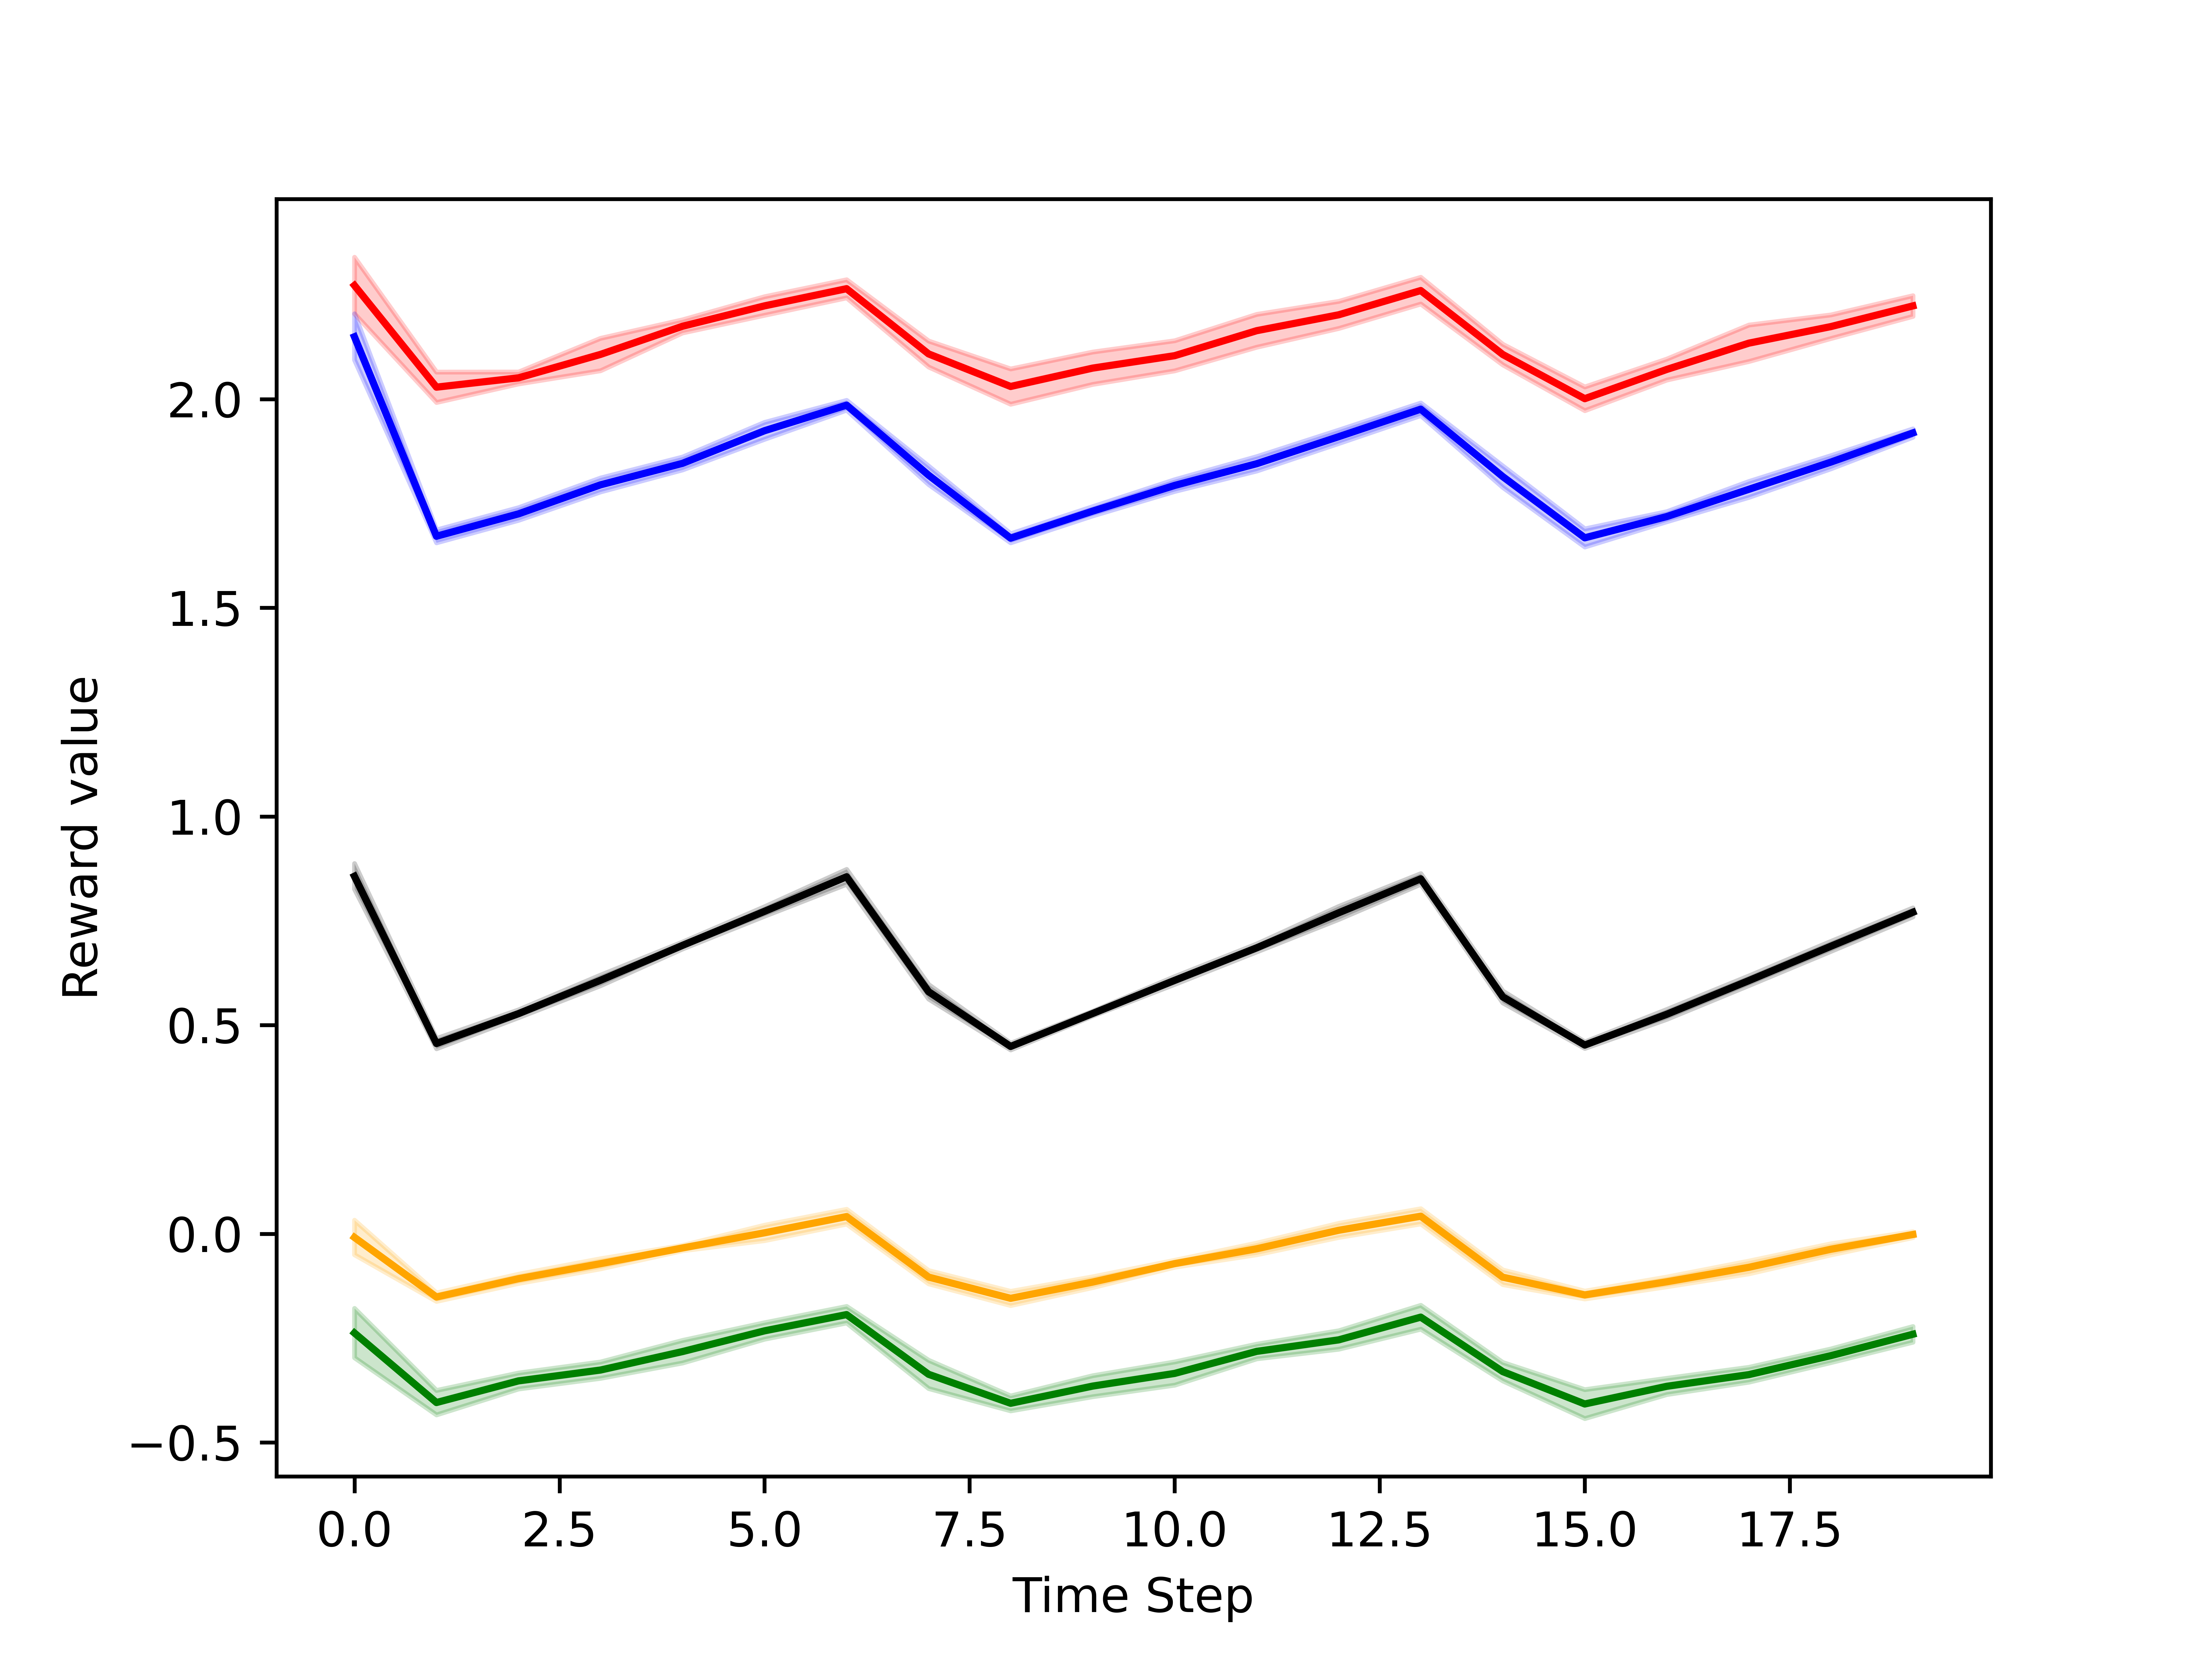
\includegraphics[width= 0.95\linewidth,clip]{1200_07}
		\caption{$\alpha_p=0.7$, relative speed-up of \num{1.9\pm0.2} for partial expectation and \num{1.2\pm0.2} for SITH}
		\label{fig:alpha_07}
	\end{subfigure}
	\caption{Bounds on the Boer's estimator for $\alpha_s=\alpha_p^2$, averaged over 10 runs using a nominal 1200 belief particles.}
	\label{fig:boers_bound_comp}
\end{figure}
	From \cref{fig:boers_bound_comp}\footnote{The periodic nature of the plots is a results of the periodic definition of the observation covariance in the simulations which can be noticed in \cref{fig:belief_trajectory}.} it is apparent that as $\alpha$ shrinks both bounds become looser, as is expected, but that the bounds of SITH loosen more than our bounds. In all cases our lower bound outperforms that of SITH. With respect to the upper bound, as we use less particles in the bound calculations, we note that our bounds begin to outperform those of SITH. In these simulations we defined $\alpha_s=\alpha_p^2$ and use the same $n$ particles between bounds. The idea was to keep the speed-up constant between the algorithms and compare for bound tightness. What we see though is that even though the same particles are used, our bounds still outperform those of SITH with respect to speed-up, almost by a factor of two at times, while supplying comparable bounds, if not better. Finally we would like to note that for larger values of $\sigma_{\observation{}{}}$ (we found this to be about $\sigma_{\observation{}{}}>r_{\action{}}+r_{\observation{}{}}$), the SITH upper bound would becomes superfluous, returning $\infty$. This is due to the upper bound of $(b)$ in Theorem 3. of~\cite{Sztyglic22iros} which is a summation of the transition likelihood between a subset of prior particles and all propagated particles. As we use a particle filter, nothing ensures that a propagated particle will have a prior particle with non-zero transition likelihood because of the truncated Gaussian. This problem is avoided in our bounds as the summation is between a subset of prior particles and the propagated subset itself.
\section{High Dimensional Planning}
\subsection{Simulation Setup}
\begin{figure}[h]
	\centering
	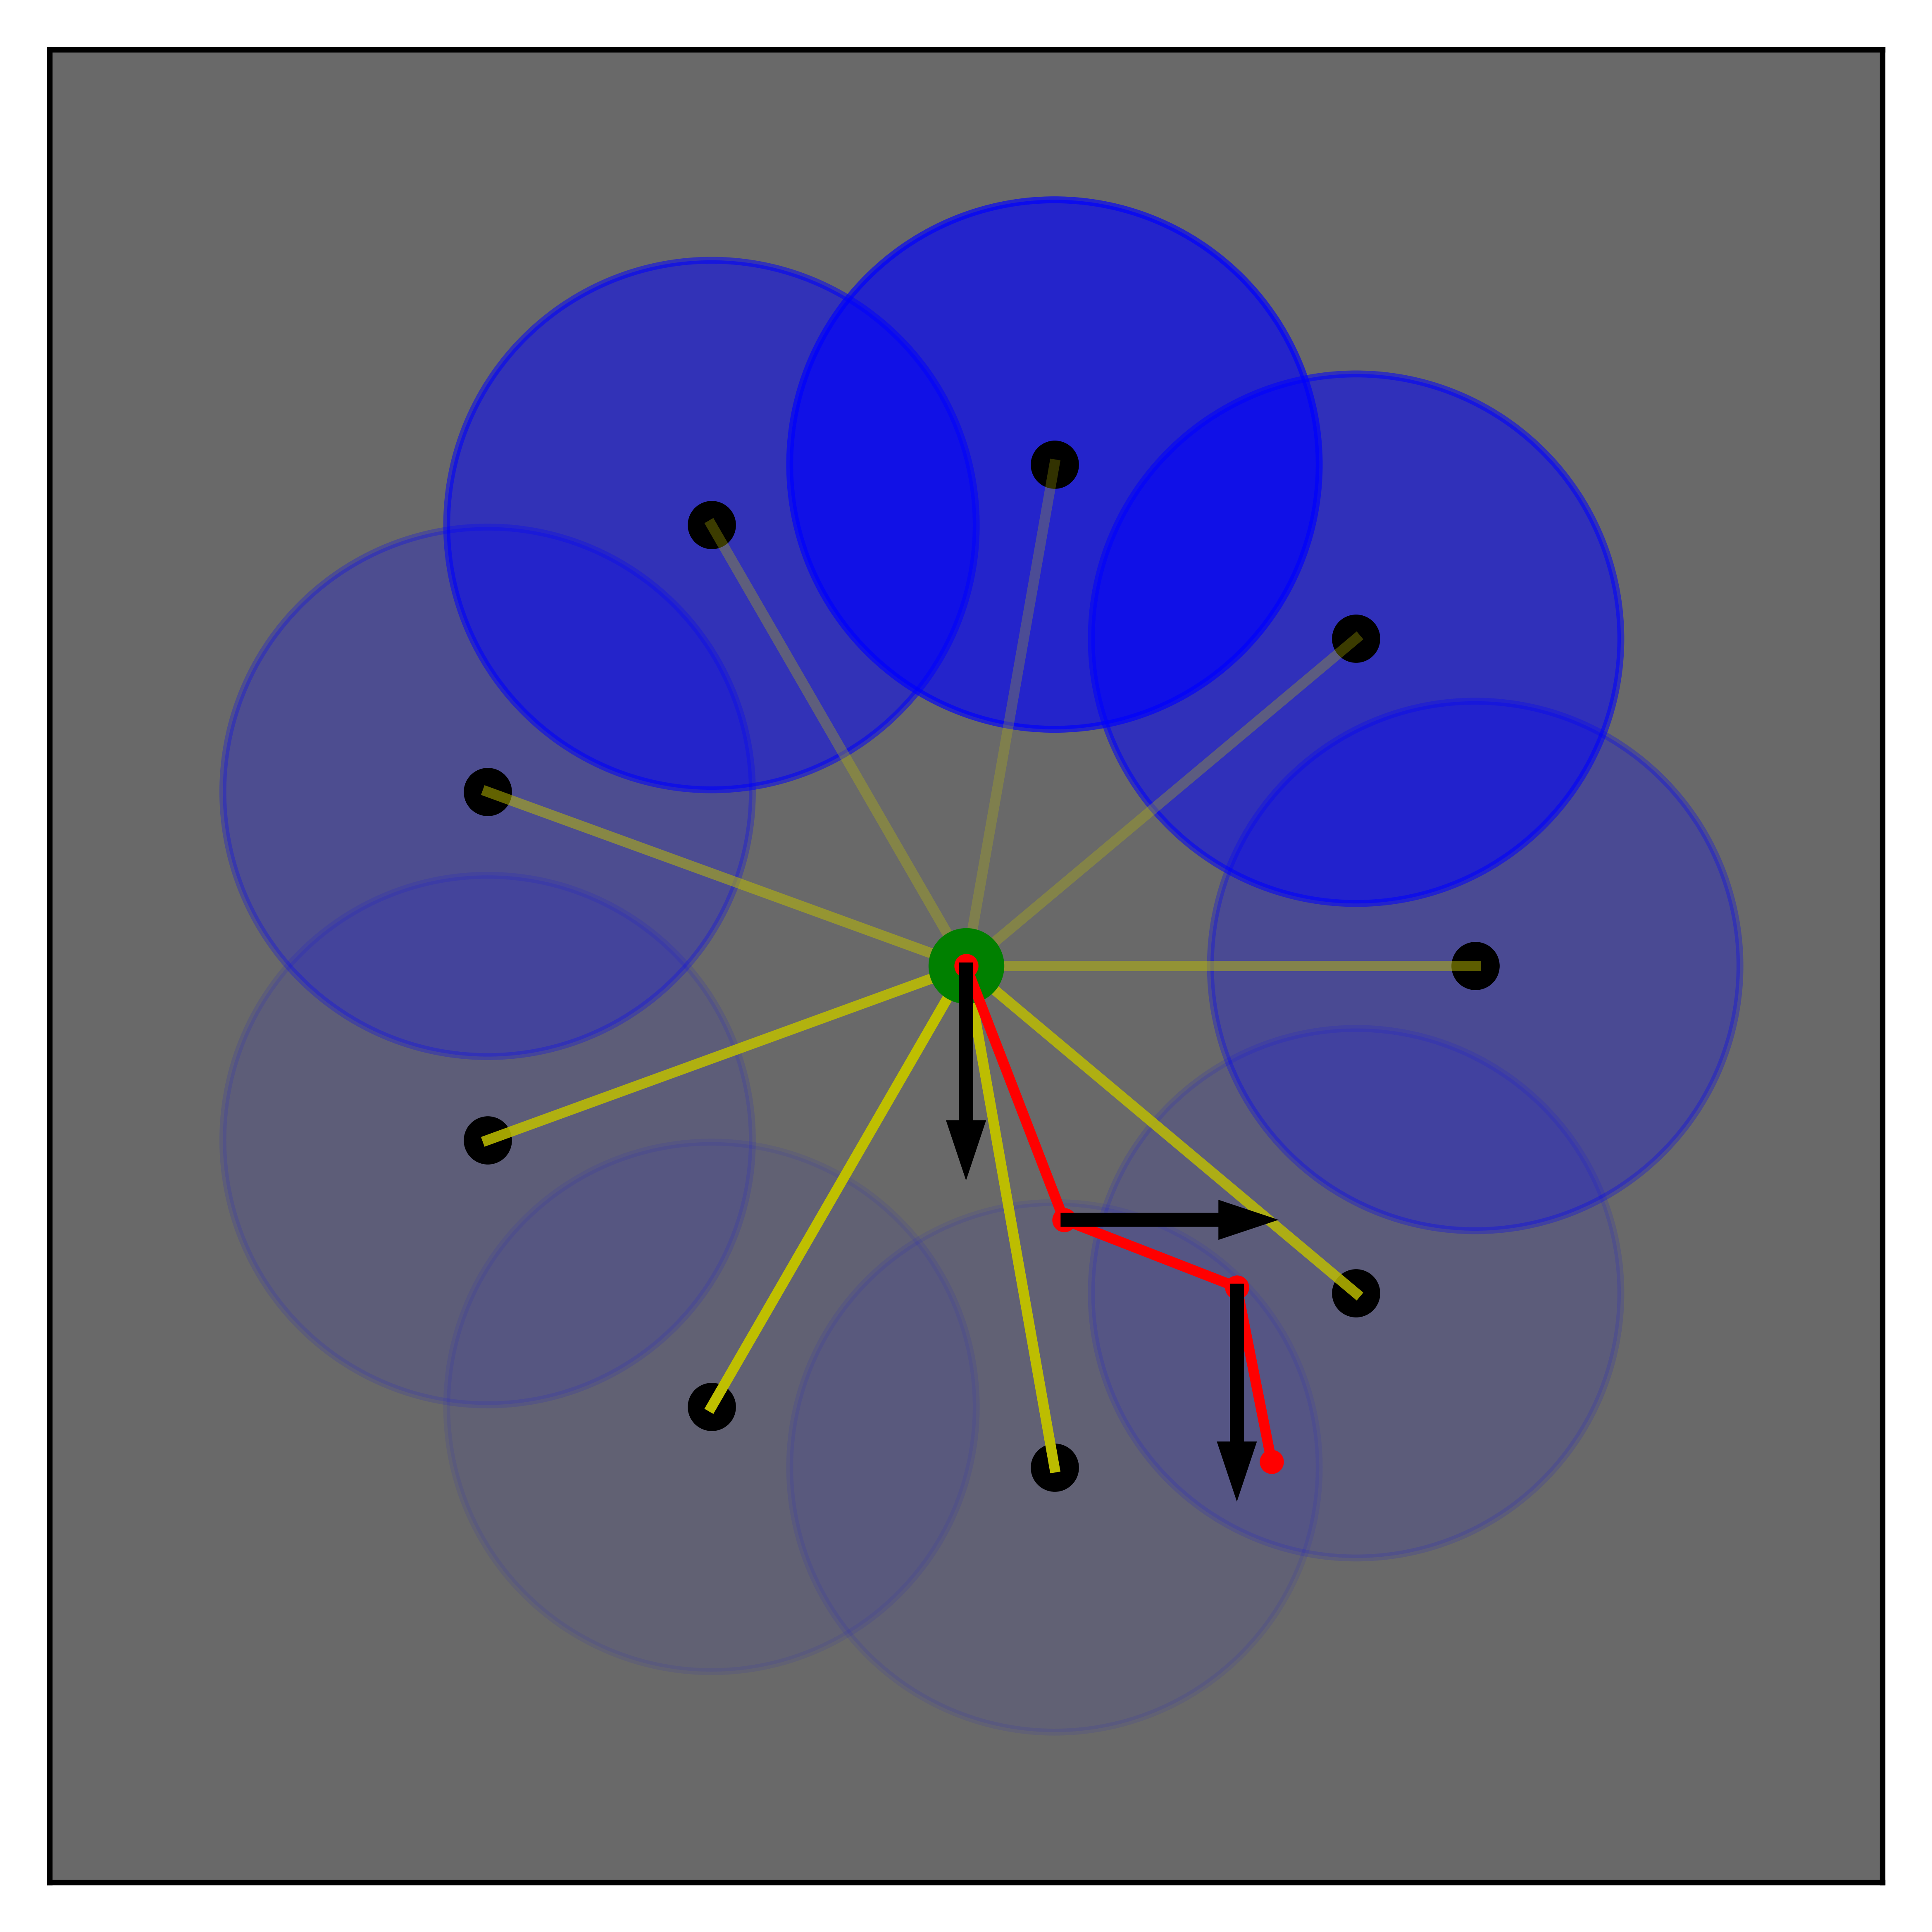
\includegraphics[width= 0.4\linewidth,clip]{actions}
	\caption{The agent path as dictated by the optimal actions, overlayed with the actions selected by the maximum lower bound on the Q-function for $\kappa=0.5$. In this case the maximum lower bound was in agreement with the optimal action, this is not always the case. The beacon intensity denotes its probability of success. And the line intensities are directly proportional to the covariance of the observation factor used as an initial belief.}
	\label{fig:actions}
\end{figure}
As discussed in \cref{sec:complete_elimination}, \autoref{thm:bounds_elim} can be utilized alongside \eqref{eq:remove_da} when formulated for expected reward. The following simulations demonstrate the improvement in runtime and the resulting bounds obtained upon utilizing the aforementioned inequalities.

We consider planning in the landmark-\gls{slam} scenario, a high-dimensional smoothing problem where the state space expands over time to include current and past poses, as well as landmarks in $\mathbb{R}^2$. The action space consists of unit circle motion primitives. The transition model is given by $\state{}^\prime=\state{}+\action{}+\omega_{\action{}}$ where $\omega_{\action{}}\sim N_{r_a}(0,I\sigma_{\action{}}^2)$, and the observation model is given by $\observation{}{}=\landmark{}-\state{}+\omega_{\observation{}{}}$, where $\omega_{\observation{}{}}\sim N_{r_{\observation{}{}}}(0,I\sigma_{\observation{}{}}^2)$. Observations are relative position between poses and landmarks. Each landmark $\landmark{i}$ has probability $p_i$ to succeed in sending an observation to the agent once the agent is within a radius $r$ of the landmark (i.e. $\probcond{\da{}{i}}{\state{},\landmark{i}}=\1{\norm{\state{}-\landmark{i}}\leq r}p_i$). The reward is given to be negative entropy as the task is information gain.

An initial belief over the agent pose and landmarks is instantiated via a prior on the initial pose and observation factors to each landmark. Subsequently belief tree is constructed using sparse sampling, where, in addition to action and observation nodes, we introduce \gls{da} nodes (see \cref{fig:topology}). High-dimensional inference is handled incrementally using the slices approach from~\cite{Shienman24arxiv}. After constructing the tree in a downward pass, rewards, expected reward bounds, and Q-functions are calculated in an upward pass while maintaining Bellman optimality. In the case of bounds on the Q-function, the maximum over the lower and upper bounds are passed up. We define $\kappa$ as $\frac{\abs{\subSpace}}{\abs{\mathcal{D}}}$, representing the proportion of \gls{da} nodes eliminated for the expected reward bounds.  When $\kappa=1$ no nodes are eliminated and the expected reward remains unchanged; for $\kappa=0$ all $\da{}{}$ realizations are discarded, resulting in loose bounds on the expected reward. Specifically, $\kappa$ splits $\mathcal{D}$ into two sets: $\da{}{}\in\subSpace$ and $\tilde{\da{}{}}\in\stcomp{\subSpace}$ as required for \autoref{thm:bounds_elim}. The reference \gls{da}, $\da{}{}$, is used to calculate bounds on $\condEntropy{\statesRV{}}{\observationsRV{},\tilde{\da{}{}}}$; the selection process of a reference \gls{da} is not addressed in this work, and we simply select a reference \gls{da} such that $\da{\textup{diff}}{}\neq0$. Joint state sampling via~\cite{Shienman24arxiv} allows access to the estimated joint likelihood which was used to evaluate the reward. The weighted samples represent our belief over the state for reward calculations, using the same samples for both rewards and bounds.

\subsection{Results}
\begin{figure}[h]
	\centering
	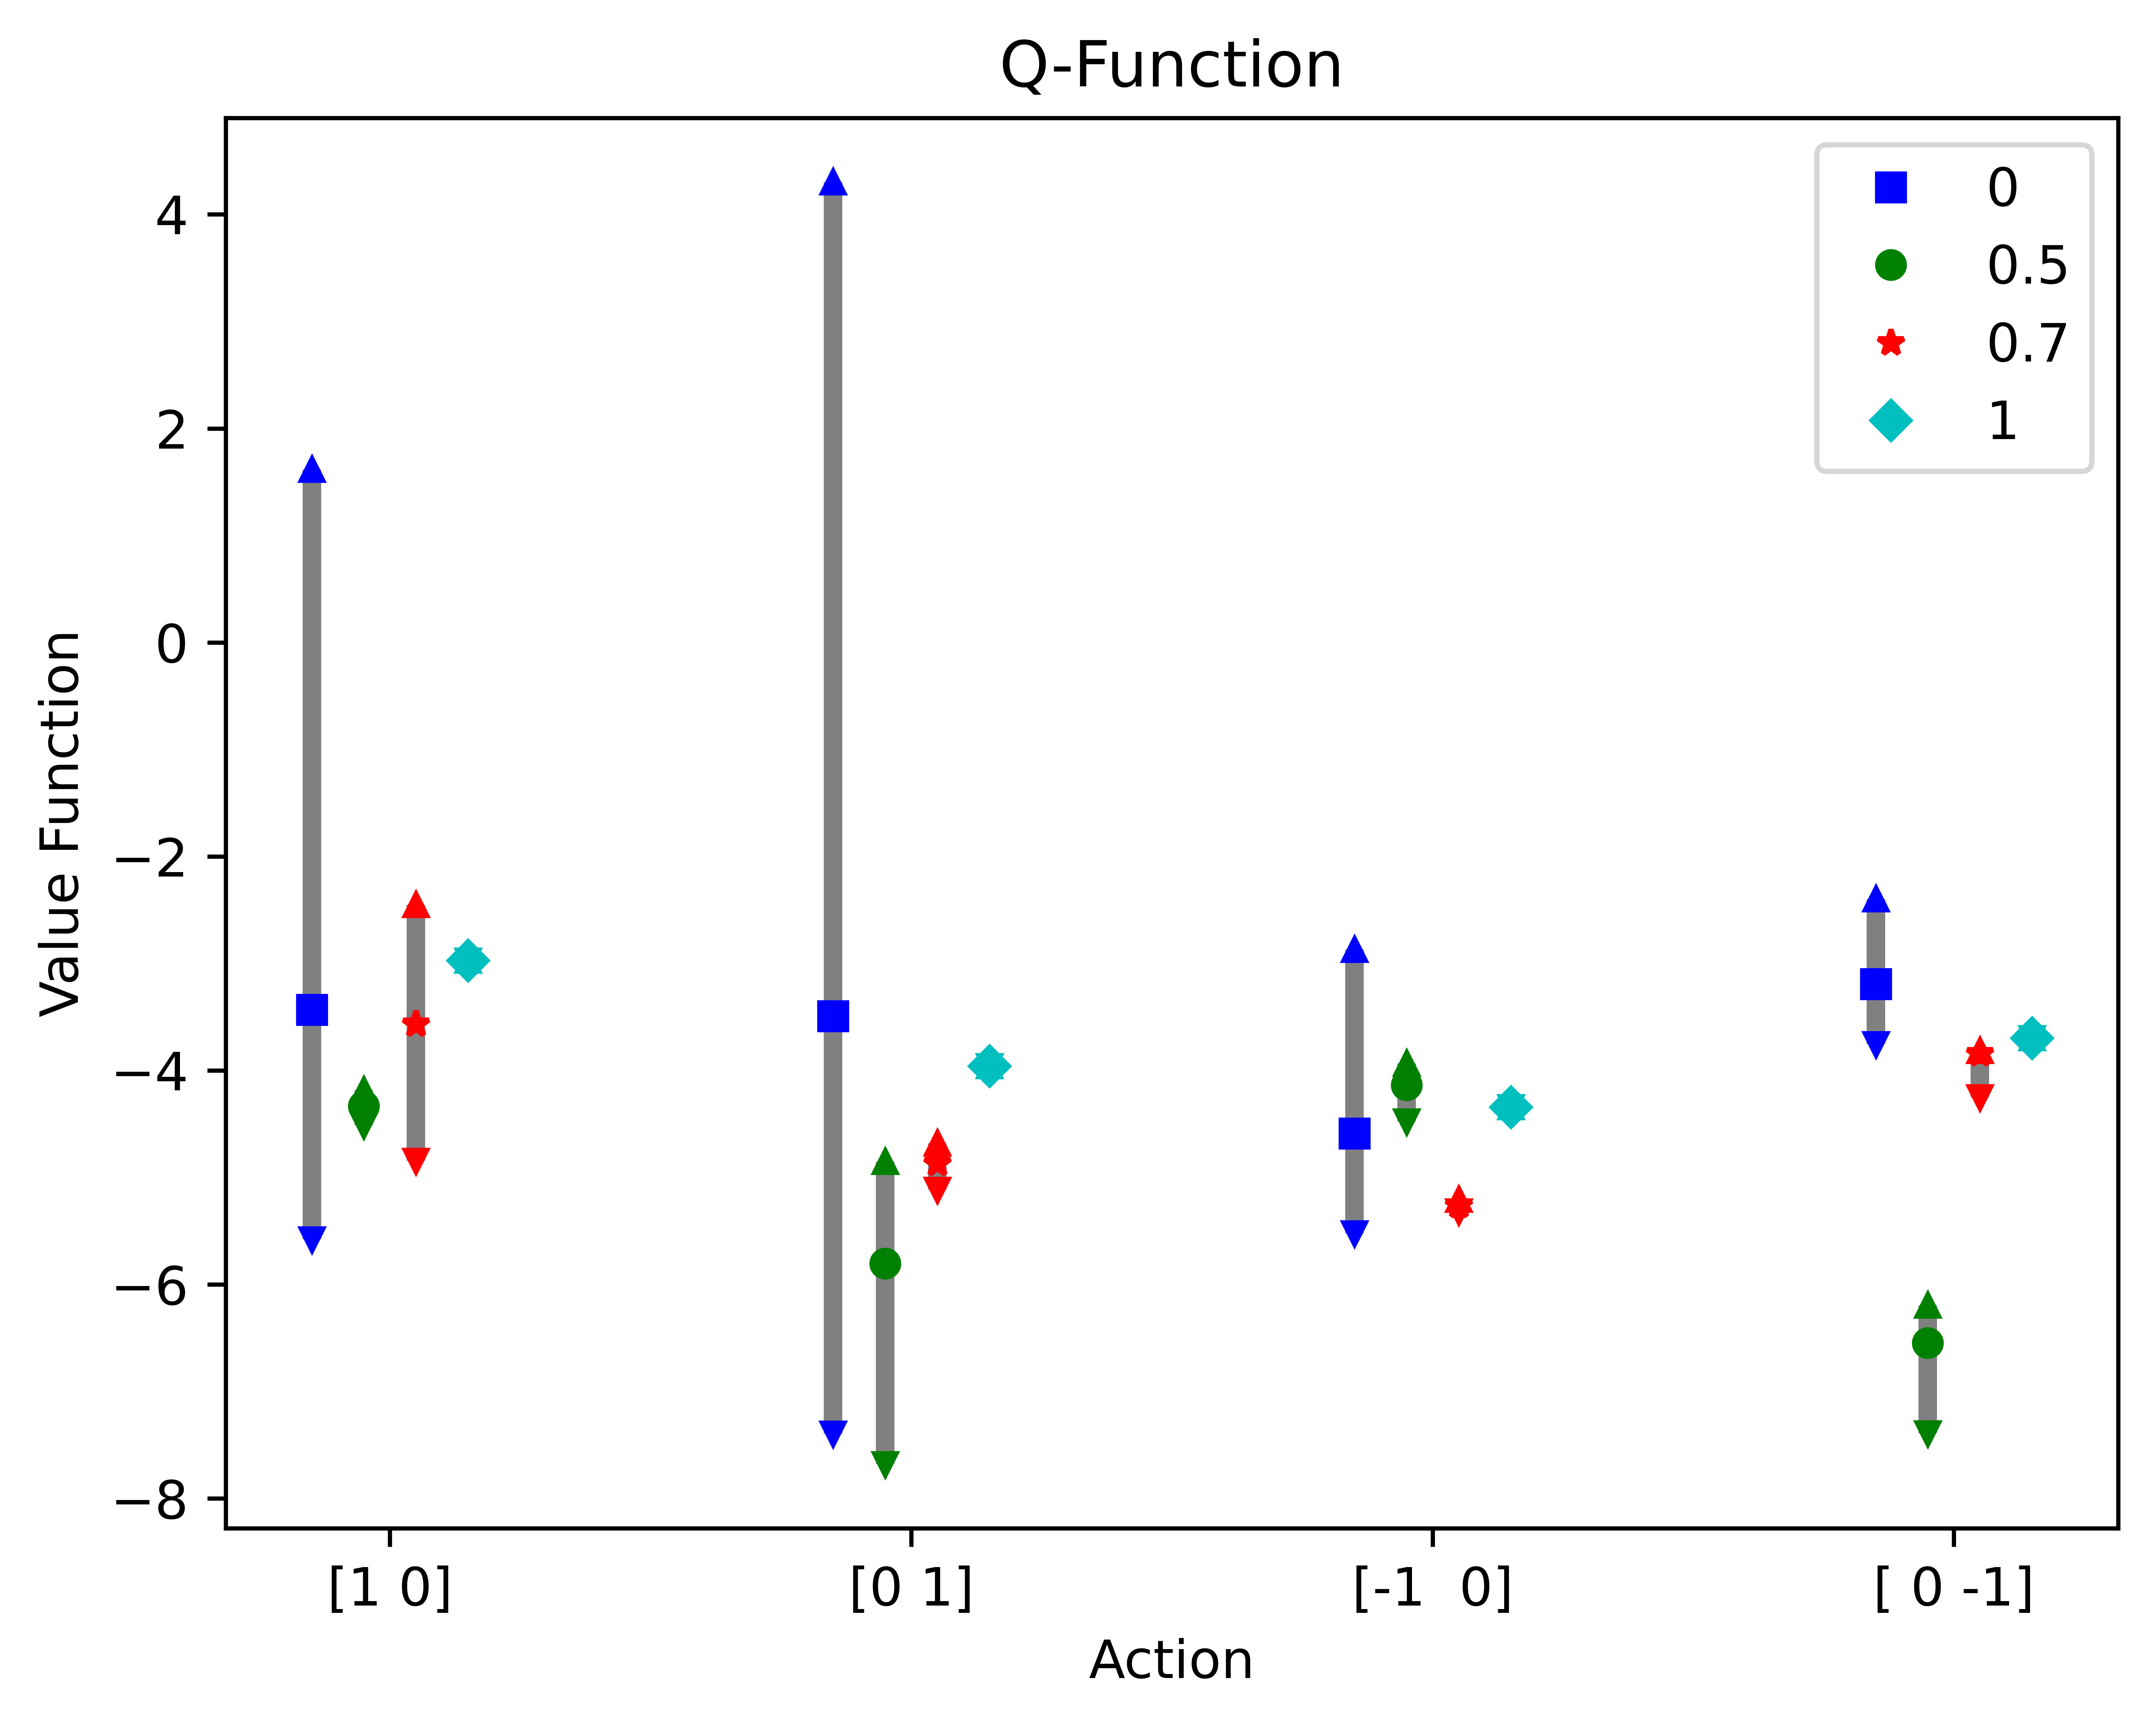
\includegraphics[width= 0.4\linewidth,clip]{q_function}
	\caption{Comparison of the Q-functions alongside the bounds calculated on the Q-functions for various values of $\kappa$.}
	\label{fig:q_function}
\end{figure}
From \cref{fig:q_function} we first note that for $\kappa=0$ the bounds are most loose, but offer a significant speedup as shown if \cref{table:results}. In essence, these are the free bounds. For $\kappa=1$ we find that the bounds converge to the optimal Q-function and no penalty is suffered to the speedup. Finally for $\kappa=\numlist{0.5;0.7}$ we observe a speedup of $\times$\numlist{2.6;1.3} respectively. Although the bounds on the Q-function overlap in both cases, not permitting optimal action selection, they do allow for action elimination. For $\kappa=0.7$ actions \numlist{2;3} can be eliminated, for $\kappa=0.5$ actions \numlist{2;4} can be eliminated. The Q-function bounds for a given $\kappa$ differ in looseness as the bounds are proportional to $\measure{\stcomp{\subSpace}}$ and so depend on the \gls{da} eliminated. As higher weighted \gls{da} nodes are discarded, the bounds are proportionally weighted, the benefit being that often times \gls{da} nodes with higher likelihood must be traversed more times for evaluating the reward. Finally, as the number of \gls{da} nodes per action is limited in our simulation, often times we must take $\da{\textup{ref}}{}=0$, as for all other $\da{\textup{ref}}{}$ $\da{\textup{diff}}{}=0$. Finally, due to the discrete nature of the division of $\mathcal{D}$, as $\abs{\mathcal{D}}$ grows, the value of $\frac{\abs{\subSpace}}{\abs{\mathcal{D}}}$ approaches the pre-defined $\kappa$.
\begin{table}
	\centering
	\caption{A value of $q=2$ was selected for \autoref{thm:bounds_elim}. 150 samples were used for inference, 150 observations per action for sparse sampling, and 100 samples for reward calculations.}\label{table:results}
	\scalebox{0.8}{
	\begin{tabular}{|c|c|c|c|c|}
		\hline
		$\kappa$\tablefootnote{results are averaged over three runs.}&  No. Eliminated Factors & Reward Runtime [\unit{\second}] & Bounds Runtime [\unit{\second}] & Speedup \\
		\hline
		\num{1} & \num{0\pm 0} & \num{876.5 \pm164.5} & \num{874.0\pm 164.5} & \num{1.0\pm0.0} \\
		\hline
		\num{0.7} & \num{88\pm 45} & \num{991.1 \pm446.6} & \num{743.7\pm 283.4} & \num{1.3\pm0.1} \\
		\hline
		\num{0.5} & \num{189\pm 92} & \num{720.8 \pm43.0} & \num{295.0\pm 94.5} & \num{2.6\pm0.4} \\
		\hline
		\num{0} & \num{330\pm 164} & \num{651.7\pm123.5} & \num{16.3\pm 0.6} & \num{39.8\pm7.1} \\
		\hline
	\end{tabular}}
\end{table}

